\documentclass{amsart}

\usepackage[utf8]{inputenc}
\usepackage[margin=.9in]{geometry}

\usepackage[]{amsmath}
\usepackage{amsthm}
\usepackage{latexsym}
\usepackage{amssymb}
\usepackage{mathrsfs}
\usepackage{exscale}
\usepackage{textcomp}
\usepackage[all,ps,tips,tpic]{xy}
\usepackage{upgreek}
\usepackage{url}
\usepackage{booktabs}
\usepackage[final,pdftex,colorlinks=false,pdfborder={0 0 0}]{hyperref}
\usepackage{microtype}
\usepackage{verbatim}
\usepackage{soul}
\usepackage{tikz}
\pagenumbering{gobble}

\theoremstyle{definition}
\newtheorem*{example*}{Example}
\newcommand{\sd}{\operatorname{\mathrm{sd}}}

%spacing around left-right brackets
\let\originalleft\left
\let\originalright\right
\renewcommand{\left}{\mathopen{}\mathclose\bgroup\originalleft}
\renewcommand{\right}{\aftergroup\egroup\originalright}

\begin{document}
\title{Documentation: tournser}

\author{Jason P. Smith}
\address{University of Aberdeen, Aberdeen, United Kingdom}
\email{jason.smith@abdn.ac.uk}

\maketitle

\noindent
The software \textsc{tournser} is designed for the computation of persistent
homology for tournaplexes with different filtrations, see for \href{https://arxiv.org/abs/2003.00324}{here} for the background.
\textsc{Tournser} is an adaptation of \href{https://github.com/luetge/flagser}{\textsc{flagser}}
 which in turn is an adaptation of Ulrich Bauer's
\href{https://github.com/Ripser/ripser}{\textsc{ripser}}.
An online version of tournser is available \href{https://homepages.abdn.ac.uk/neurotopology/tournser.html}{here}.


\section{Compiling the source code}
\noindent
\textsc{Tournser} requires a C++14 compiler.
For Linux or Mac (Windows is currently not supported) open the terminal, change into the \textsc{tournser} main directory and execute

\vspace{1em}

\begin{verbatim}c++ tournser.cpp -o tournser -std=c++14 -pthread -O3\end{verbatim}

\vspace{1em}

\section{Usage}
\noindent
After building \textsc{tournser}, you can compute persistent homology as follows:

\vspace{1em}

\begin{verbatim}./tournser in_file_address out_file_address [options]\end{verbatim}

\vspace{1em}

For example:

\vspace{1em}

\begin{verbatim}./tournser ./Examples/test.trn ./Examples/test.homology --filtration relative\end{verbatim}

\vspace{1em}

\noindent
The following \texttt{[options]} exist:

\enlargethispage{\baselineskip}
\begin{description} 
  \item [-{}-filtration] One of the following which gives filtration value $F(\sigma)$ to simplex $\sigma$:
  \begin{itemize}
    \item \emph{local}: $F(\sigma)=2\binom{n}{3}+\sum_{v\in \sigma}(\sd_\sigma(v))^2$
    \item \emph{global}:  $F(\sigma)=\sum_{v\in \sigma}(\sd_\mathcal{G}(v))^2$
    \item \emph{3cycle}: $F(\sigma)=$ Number of directed 3-cycles in $\sigma$
    \item \emph{vertexMax}: $F(\sigma)=\max_{v\in\sigma}(F(v))$
    \item \emph{vertexSum}: $F(\sigma)=\sum_{v\in\sigma}F(v)$
    \item \emph{natural}: $F(\sigma)=\sum_{v\in \sigma}(\sd_\sigma(v))^2+\max_{b\in bdry(\sigma)}F(b)$
    \item \emph{natural-max}: $F(\sigma)=\max(\sum_{v\in \sigma}(\sd_\sigma(v))^2,\max_{b\in bdry(\sigma)}F(b))$
  \end{itemize} 
  where $sd_X(v)=indeg_X(v)-outdeg_X(v)$ and $indeg_X(v)$ is the indegree of vertex $v$ in the digraph $X$.
  \item [-{}-max-dim \textit{dim}] the maximal homology dimension to be computed
  \item [-{}-min-dim \textit{dim}] the minimal homology dimension to be computed
  \item [-{}-print\_dist true] Prints the distribution of the filtration values
  \item [-{}-count\_only true] Computes only the simplex counts and skips all homology computations
  \item [-{}-print print\_address] Prints the whole tournaplex to a file, see below for format.
  \item [-{}-approximate \textit{n}] skip all cells creating columns in the reduction matrix with
    more than $n$ entries. Use this for hard problems, a good value is often 100000. Increase for
    higher precision, decrease for faster computation. This function is taken from \textsc{flagser}, see for \href{https://www.mdpi.com/1999-4893/13/1/19}{this article} more information.
\end{description}

\vspace{1em}

\newpage
\subsection{Input Format}

\noindent
The input file defines the directed graph and must have the following shape:

\vspace{.5em}
\begin{verbatim}
dim 0:
weight_vertex_0 weight_vertex_1 ...  weight_vertex_n
dim 1:
first_vertex_id_of_edge_0 second_vertex_id_of_edge_0 [weight_edge_0]
first_vertex_id_of_edge_1 second_vertex_id_of_edge_1 [weight_edge_1]
...
first_vertex_id_of_edge_m second_vertex_id_of_edge_m [weight_edge_m]
\end{verbatim}
\vspace{.5em}

\noindent
The edges are oriented to point from the first vertex to the second vertex, the weights of the edges
are optional.
The weights should be rational numbers.
Important: the input graphs can not contain self-loops, i.e.\ edges that start and end in the same vertex.

\begin{example*}
  The full directed graph on three vertices without explicit edge weights is described by the
  following input file:

  \vspace{.5em}
  \begin{verbatim}
  dim 0:
  0.2 0.522 4.9
  dim 1:
  0 1
  1 0
  0 2
  2 0
  1 2
  2 1
  \end{verbatim}
\end{example*}


\subsection{Print Tournaplex}
Using the option \textbf{-{}-print print\_address} will print the whole tournaplex to a file, where each simplex is written as a line with the following information:
  \begin{itemize}
    \item \emph{Vrts}: This is the vertices of the simplex
    \item \emph{bdry}: This is the boundary of the simplex, where each number corresponds to the simplex in the dimension below which has that ``loc" value
    \item \emph{cbdry}: This is the coboundary of the simplex, where each number corresponds to the simplex in the dimension above which has that ``loc" value
    \item \emph{filt}: The filtration value of the simplex
    \item \emph{ort}: The orientation of the edges of the tournament represented as a lower triangular matrix $M$, where the first entry is $M_{1,0}$ and each row is separated by :,
     where $$M_{i,j}=\begin{cases}0,&\mbox{ if }i\rightarrow j\\1,&\mbox{ if }i\leftarrow j\end{cases}$$
    \item \emph{loc}: The location (or index) of the simplex, i.e all simplices in dimension $k$ are numbered $0$ to $n_k$.
  \end{itemize}
  For example:
  \begin{verbatim}
    Vrts = 0 1 3 | bdry = 5 2 3 | cbdry = 1 3 | ort = 0 : 1 1 : | filt = 4 | loc = 5
  \end{verbatim}
  Corresponds to the simplex in dimension 2 which is given by the tournament $$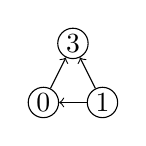
\begin{tikzpicture}[scale=.75]
	\node[circle, draw=black,inner sep=1pt] (0) at (0,0){$0$};
	\node[circle, draw=black,inner sep=1pt] (1) at (1,0){$1$};
	\node[circle, draw=black,inner sep=1pt] (3) at (.5,1){$3$};
	\draw[->] (1) -- (0);
	\draw[->] (0) -- (3);
	\draw[->] (1) -- (3);
   \end{tikzpicture}$$
  and this simplex has three faces in its boundary and two in its coboundary, has filtration value $4$ and is the $5$'th face of dimension 2

\vfill
\end{document}